% =============================================================================
% onda_vs_calor_fonones.tex — Nota teórica complementaria: sonido (ecuación
% de onda) vs. calor (ecuación de difusión) en la superficie tras el
% impacto, organizada alrededor del criterio de Gonzalo Gutiérrez: energía
% coherente produce trabajo, incoherente no (segunda ley / exergía). Incluye
% el régimen intermedio de sonido difuso (Weaver 1984) entre sonido
% balístico y calor genuino, y el número de Knudsen medido contra la
% bibliografía (Kaburaki et al. 1998).
% Compilar: pdflatex onda_vs_calor_fonones.tex (dos pasadas)
% =============================================================================
\documentclass[11pt,a4paper]{article}

\usepackage[utf8]{inputenc}
\usepackage[T1]{fontenc}
\usepackage[spanish,es-nodecimaldot]{babel}
\usepackage[margin=2.3cm]{geometry}
\usepackage{amsmath,amssymb}
\usepackage{booktabs}
\usepackage{enumitem}
\usepackage{xcolor}
\usepackage{graphicx}
\usepackage[colorlinks=true,linkcolor=blue!50!black,citecolor=blue!50!black]{hyperref}

\newcommand{\eps}{\varepsilon}
\newcommand{\kb}{k_B}
\newcommand{\lammps}{\textsc{Lammps}}
\newcommand{\clave}[1]{\textcolor{red!55!black}{\textbf{#1}}}

\title{\textbf{Sonido y calor: dos destinos de la misma energía}\\
\large Por qué el sonido del impacto es trabajo disponible, el calor no lo
es, y qué haría falta para ver a uno convertirse en el otro}
\author{Felipe Wasaff}
\date{Julio 2026}

\begin{document}
\maketitle

\begin{abstract}
En la reunión de julio 2026, Gonzalo Gutiérrez propuso mirar esto con el
vocabulario de la física clásica, no de fonones: la superficie tras el
impacto debería mostrar sonido (ecuación de onda) cerca del frente que
recién llega, y calor (ecuación de difusión) más atrás, cerca del punto de
impacto, donde la energía tuvo más tiempo para dispersarse. Y añadió el
criterio de fondo: \emph{energía coherente puede producir trabajo; energía
incoherente no puede}. Esta nota reordena el documento anterior alrededor
de esa idea --que resulta ser, literalmente, la segunda ley de la
termodinámica en su forma de disponibilidad/exergía (Kelvin 1852, Gibbs
1873, Keenan 1932, Rant 1956)--, agrega un tercer régimen intermedio que
la bibliografía sí reconoce (sonido \emph{difuso}: disperso por dispersión
múltiple, pero todavía no calor, Weaver 1984, Aki y Chouet 1975), y
contrasta todo contra lo que medimos en \texttt{ondas\_N79\_libre}:
confirmamos sonido balístico limpio ($r_{\rm frente}\propto t^{1.06}$), una
señal ambigua que ahora leemos como el borde de la región de sonido difuso,
y ninguna evidencia todavía de calor genuino --consistente con un número de
Knudsen $\sim1$--$5$ calculado de forma independiente (Kaburaki, Li y Yip
1998).
\end{abstract}

\tableofcontents

% =============================================================================
\section{La pregunta}
% =============================================================================

Un sólido que vibra transporta energía de dos maneras cualitativamente
distintas:

\begin{itemize}[leftmargin=1.4em]
\item \textbf{Sonido (ecuación de onda).} Un pulso elástico viaja
coherente, a la velocidad de grupo de los modos que lo componen, sin
perder memoria de su fase ni de su dirección. La descripción es
$\partial_t^2 u = c^2\nabla^2 u$: mecánica pura, en principio reversible.
\item \textbf{Calor (ecuación de difusión).} Después de suficiente
dispersión, la energía pierde coherencia de fase y de dirección; lo que
queda es un campo de temperatura local que obedece $\partial_t T =
D\nabla^2 T$ (ley de Fourier): termodinámica, irreversible, con
producción de entropía.
\end{itemize}

No son dos fenómenos independientes que coexisten en paralelo: son la
\emph{misma} energía vibracional vista en dos regímenes distintos del
mismo proceso microscópico. Pero la diferencia entre ambos no es solo
matemática (qué ecuación diferencial obedecen) --es la diferencia que
importa en termodinámica entre lo que puede y lo que no puede producir
trabajo, y esa es la forma más honesta de plantear la pregunta.

% =============================================================================
\section{Energía coherente y trabajo: la segunda ley de fondo}
\label{sec:segunda_ley}
% =============================================================================

El criterio que Gonzalo puso sobre la mesa --\emph{energía coherente puede
producir trabajo, energía incoherente no puede}-- no es una metáfora: es,
literalmente, el enunciado de Kelvin-Planck de la segunda ley, en la forma
en que la termodinámica de ingeniería lo formaliza desde hace más de 170
años.

\textbf{Thomson (Lord Kelvin, 1852)} \cite{Kelvin1852} fue el primero en
plantearlo con precisión: ``aunque la energía mecánica es indestructible,
hay una tendencia universal a su disipación, que produce el aumento
gradual y la difusión del calor, el cese del movimiento, y el agotamiento
de la energía potencial en todo el universo material''. Es la primera
formulación de lo que hoy llamamos segunda ley: la energía \emph{mecánica}
(coherente, ordenada, capaz de mover un pistón o hacer girar una rueda) se
degrada espontáneamente hacia energía \emph{térmica} (incoherente,
desordenada), pero no al revés --sin costo adicional.

\textbf{Gibbs (1873)} \cite{Gibbs1873} le dio forma cuantitativa concreta
al concepto de ``energía disponible'' de Thomson mediante lo que hoy se
conoce como energía libre de Gibbs. \textbf{Keenan (1932)} \cite{Keenan1932}
lo llamó \emph{availability} (disponibilidad) en el contexto de ingeniería
de turbinas de vapor, y \textbf{Rant (1956)} \cite{Rant1956} acuñó el
nombre que se usa hoy: \textbf{exergía} --del griego \textit{ex} (``desde'')
y \textit{ergon} (``trabajo'')--, definida como el máximo trabajo que se
puede extraer de un sistema al llevarlo al equilibrio con su entorno. La
energía total se separa así en dos partes,
\begin{equation}
E = \underbrace{\rm Ex}_{\text{exergía: capaz de trabajo}}
    + \underbrace{\rm An}_{\text{anergía: no capaz de trabajo}},
\label{eq:exergia}
\end{equation}
y el resultado central de la segunda ley es que la exergía \emph{solo puede
disminuir} en un proceso irreversible --nunca aumenta--, mientras que la
energía total, por supuesto, se conserva siempre.

\textbf{Esto es exactamente el eje de este documento, en otro lenguaje.} Un
pulso de sonido coherente --el frente balístico del impacto-- es, en el
sentido de Rant, casi pura exergía: en principio, con el aparato correcto
(un transductor, una turbina, un segundo cristal bien acoplado), esa
energía podría convertirse íntegramente en trabajo útil, porque todavía
``sabe'' en qué dirección moverse. El calor --velocidades atómicas
isotrópicas, sin dirección privilegiada-- es mayormente anergía: por el
teorema de Carnot, ni siquiera en el mejor de los casos se puede convertir
completamente en trabajo, solo una fracción acotada por la temperatura
del entorno. La pregunta ``¿esto es todavía sonido o ya es calor?'' es,
en el fondo, la pregunta ``¿cuánta de esta energía sigue siendo exergía?''
--y eso es precisamente lo que el criterio de anisotropía de
velocidades de la Sec.~\ref{sec:criterio} intenta medir.

% =============================================================================
\section{La ecuación de transporte de Boltzmann para fonones}
\label{sec:peierls}
% =============================================================================

El vocabulario de sonido y calor de las secciones anteriores es clásico y
suficiente para plantear la pregunta; pero para predecir \emph{cuándo}
ocurre la transición hace falta bajar al nivel microscópico --los cuantos
de vibración de la red, los fonones-- porque es ahí donde vive el
parámetro de control.

La formulación microscópica que contiene ambos límites como casos
particulares es la ecuación de transporte de Boltzmann para fonones,
formulada por primera vez por \textbf{Peierls (1929)}
\cite{Peierls1929}. Extiende la teoría cinética de un gas clásico de
partículas a un ``gas de fonones'': cada modo normal se trata como una
cuasipartícula que se propaga a su velocidad de grupo $v_g(\mathbf k)$ y
colisiona con otros fonones a una tasa gobernada por la anarmonicidad del
potencial interatómico. Sin colisiones, cada fonón simplemente viaja en
línea recta; las colisiones son las que, acumuladas, producen difusión.

\subsection{El número de Knudsen: quién manda, la onda o el calor}

El parámetro que decide cuál de las dos descripciones límite aplica es el
\textbf{número de Knudsen},
\begin{equation}
\mathrm{Kn} = \frac{\ell_{\rm fonón}}{L},
\label{eq:knudsen}
\end{equation}
el cociente entre el camino libre medio de los fonones $\ell_{\rm fonón}$
(la distancia típica que recorre un fonón entre colisiones) y el tamaño
característico del problema $L$ (aquí, la distancia al punto de impacto o
el tamaño del pulso). Esta es la forma estándar en la literatura de
transporte térmico a nanoescala \cite{Cahill2003}:
\begin{itemize}[leftmargin=1.4em]
\item $\mathrm{Kn}\gg1$: el fonón típico no colisiona en el trayecto que nos
interesa --\textbf{régimen balístico}, ecuación de onda.
\item $\mathrm{Kn}\ll1$: el fonón colisiona muchas veces --\textbf{régimen
difusivo}, ley de Fourier / ecuación de calor.
\end{itemize}
El cruce entre ambos no es abrupto: es una transición suave conforme $L$
crece (o, equivalentemente, conforme pasa más tiempo y la energía se aleja
más del punto donde se originó). Esto se ha medido experimentalmente, por
ejemplo en grafeno suspendido: discos de radio $<775$~nm muestran transporte
puramente balístico, mientras que discos más grandes muestran la transición
hacia difusivo por dispersión fonón-fonón resistiva \cite{Cahill2003}.

\begin{figure}[htb]
\centering
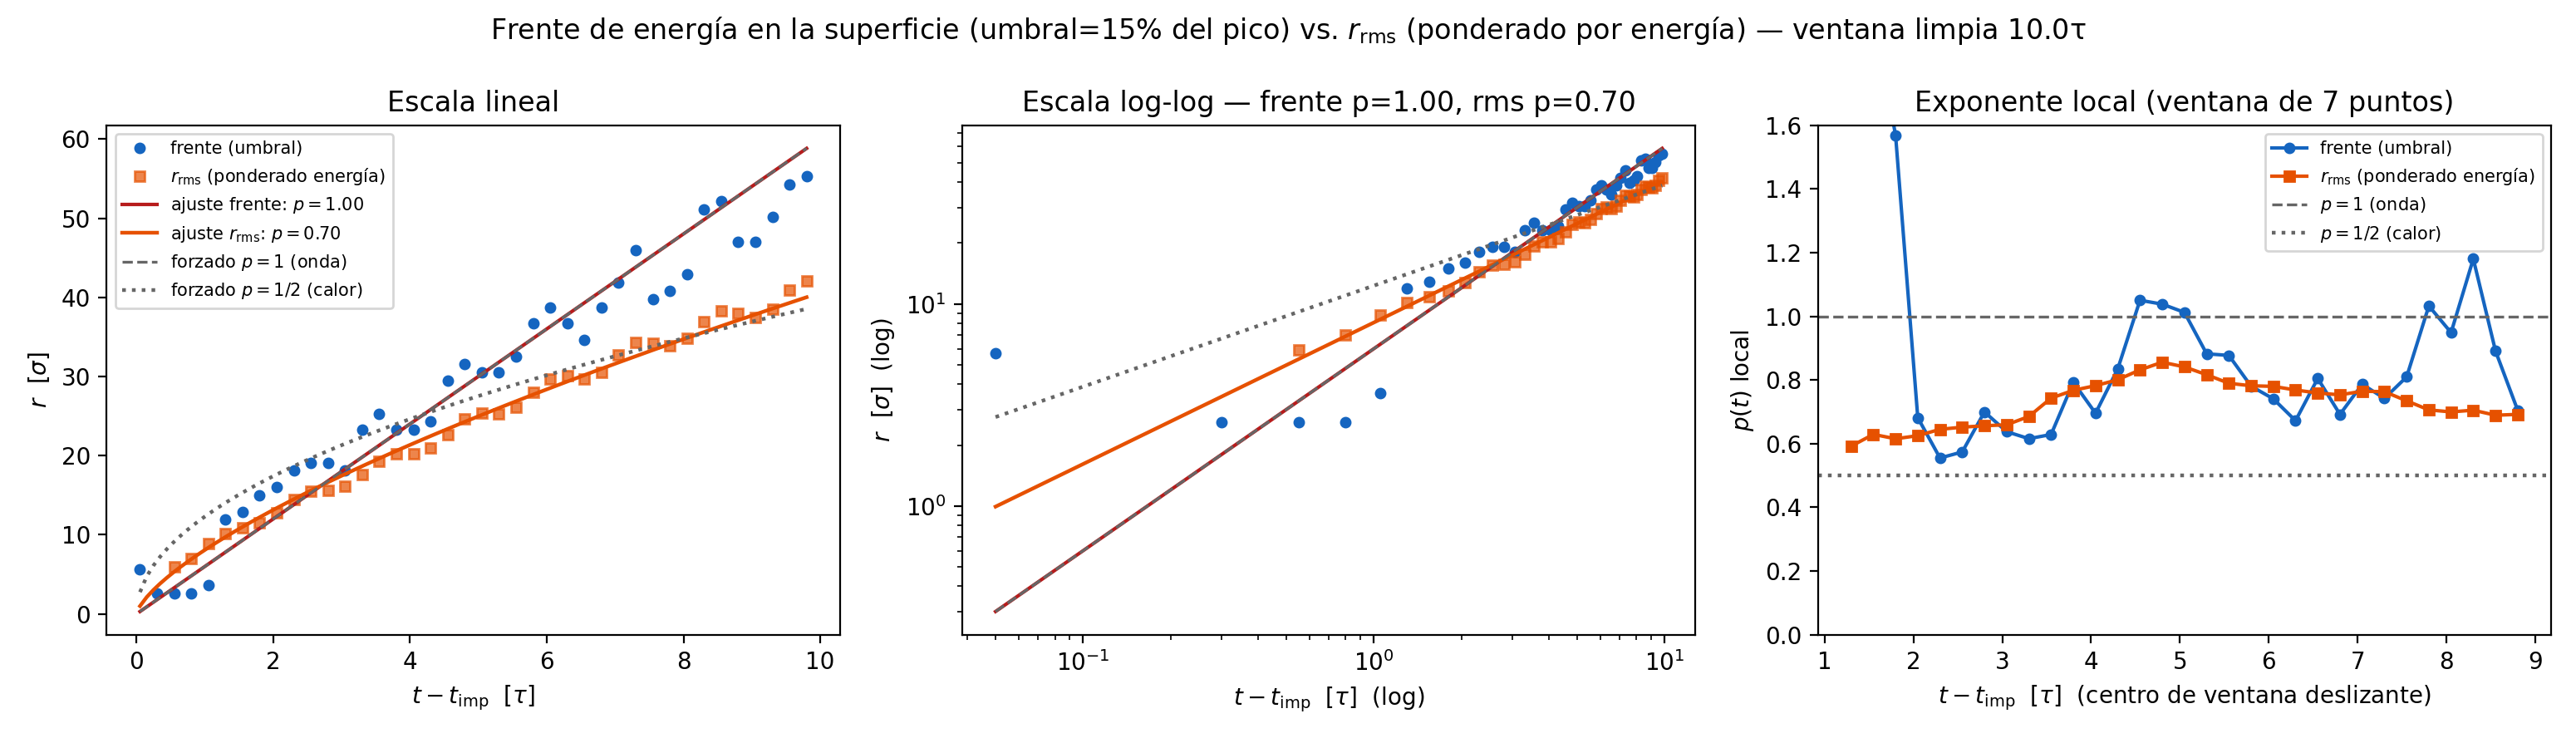
\includegraphics[width=\textwidth]{../figuras_rbef/fig_frente_onda.png}
\caption{Posición del frente de energía $r_{\rm frente}(t)$ en la ventana
limpia de \texttt{ondas\_N79\_libre} (Nx=Ny=80, sin periodicidad), medida
de dos formas: por umbral (azul, sensible al borde exterior) y por radio
cuadrático medio ponderado por energía (naranja, $r_{\rm rms}$, promedia
sobre todos los átomos y es mucho menos ruidoso). El panel derecho muestra
el exponente local $p(t)=d\ln r/d\ln t$: el frente por umbral es
consistente con $p=1$ (onda) todo el tiempo; $r_{\rm rms}$ se estabiliza en
$p\approx0.70$--$0.75$ sin tender hacia $0.5$ --ver Sec.~\ref{sec:dispersion}
para la interpretación (dispersión, no difusión).}
\label{fig:frente}
\end{figure}

% =============================================================================
\section{Por qué hace falta anarmonicidad --y por qué eso ya lo vimos}
\label{sec:armonico}
% =============================================================================

Un resultado profundo y contraintuitivo: \textbf{un cristal perfectamente
armónico no conduce calor en el sentido de Fourier, sin importar cuánto
tiempo se espere}. Rieder, Lebowitz y Lieb (1967) \cite{RLL1967}
demostraron rigurosamente, para una cadena armónica acoplada a baños
térmicos en sus extremos, que el flujo de calor en el estado estacionario es
proporcional a la \emph{diferencia} de temperatura $(T_1-T_N)$, no al
\emph{gradiente} $(T_1-T_N)/N$ como exige la ley de Fourier --es decir, la
conductividad térmica efectiva diverge con el tamaño del sistema. Sin
colisiones fonón-fonón, el transporte es balístico para siempre,
sin importar cuán grande sea el cristal.

Esto conecta directamente con algo que ya está en el proyecto
(\texttt{equiparticion\_y\_virial.tex}): la razón por la que
$\alpha_{\Delta V_B}$ excede sistemáticamente a $\alpha_{T_B}$ es la
anarmonicidad de Lennard-Jones (el parámetro de Grüneisen). Esa misma
anarmonicidad es, en el lenguaje de este documento, el mecanismo físico que
hace posible el régimen difusivo en la superficie --sin ella, ningún tiempo
de espera alcanzaría para termalizar, y solo veríamos ondas viajando para
siempre (como en el famoso experimento numérico de
\textbf{Fermi, Pasta, Ulam y Tsingou (1955)} \cite{FPU1955}: en una cadena
no lineal \emph{débilmente} anarmónica, la energía no se termaliza en el
tiempo de simulación --regresa casi por completo al modo inicial tras 157
períodos, un resultado tan inesperado que fundó el campo de la física no
lineal computacional). Lepri, Livi y Politi (2003) \cite{LLP2003} revisan en
detalle cómo la dimensionalidad y el tipo de anarmonicidad determinan si la
ley de Fourier se recupera o si la conductividad sigue divergiendo
(``transporte anómalo del calor''), incluso con anarmonicidad presente,
en redes de baja dimensionalidad.

\textbf{Consecuencia práctica para este proyecto:} no basta con esperar. Si
el camino libre medio de los fonones relevantes es mucho mayor que la
distancia que alcanzamos a observar limpiamente (antes de que la
contaminación de borde -periódica o de reflexión libre- entre en juego),
nunca veremos difusión, sin importar cuánto tiempo simulemos.

\subsection{¿Y cuánto vale ese camino libre medio? Un número, no solo una idea}
\label{sec:kn_numerico}

Esto no tiene por qué quedarse en lo cualitativo. Kaburaki, Li y Yip (1998)
\cite{Kaburaki1998} calcularon por el método de Green-Kubo el camino libre
medio de los fonones acústicos en argón sólido con el mismo potencial de
Lennard-Jones que usa este proyecto: $\ell_{\rm fonón}\approx12.2$~nm a
$T=10$~K, cayendo a $\approx3.4$~nm a $T=40$~K. Convertido a unidades
reducidas con $\sigma=3.40$~\AA{} y $\varepsilon/\kb=120$~K --los mismos
parámetros de argón que usa el proyecto (Sec. ``Convenciones'' de
\texttt{CLAUDE.md})--, ese rango de temperatura es
$T^*\in[0.083,\,0.333]$, que se superpone casi exactamente con el rango
``sólido'' de este proyecto ($T_{\rm ef}\lesssim0.20$) hasta cerca de la
fusión ($T_{\rm ef}\approx0.30$--$0.35$). El camino libre medio en esas
mismas unidades:
\begin{equation}
\ell_{\rm fonón}^* = \ell_{\rm fonón}/\sigma \;\in\; [10,\ 36]\ \sigma
\qquad\text{para } T^*\in[0.083,\,0.333].
\label{eq:ell_kaburaki}
\end{equation}
Nuestra ventana limpia (antes de que el borde contamine la señal, Fig.
\ref{fig:frente}) es de solo $\sim7.5$--$10\,\sigma$ --\textbf{del mismo
orden o menor que $\ell_{\rm fonón}^*$}. El número de Knudsen de la
Ec.~(\ref{eq:knudsen}), evaluado con estos números,
\begin{equation}
\mathrm{Kn} = \frac{\ell_{\rm fonón}^*}{L_{\rm limpio}}
\approx \frac{10\text{--}36\,\sigma}{7.5\text{--}10\,\sigma}
\sim 1\text{--}5,
\end{equation}
está en la frontera del régimen balístico o por encima de ella
($\mathrm{Kn}\gtrsim1$), nunca cómodamente por debajo de 1. Esto predice,
\emph{antes de mirar ningún dato}, exactamente lo que medimos: transporte
balístico limpio, sin señal de difusión, porque el propio tamaño de la
ventana observable es comparable al camino libre medio esperado, no mucho
mayor que él. (Advertencia: $\ell_{\rm fonón}$ de Kaburaki et al. es para
un gas de fonones en \emph{equilibrio} térmico a $T$ fija, vía Green-Kubo;
nuestro pulso es un evento transitorio fuera de equilibrio. La comparación
es de orden de magnitud, no una predicción exacta --pero es la mejor ancla
disponible en la literatura, y el orden de magnitud coincide.)

% =============================================================================
\section{El problema del diagnóstico: dispersión no es lo mismo que difusión}
\label{sec:dispersion}
% =============================================================================

Al intentar ver la sugerencia de Gonzalo directamente --¿el perfil radial
se ve ``liso'' (termalizado) cerca del impacto y ``ondulado'' (coherente)
en el frente?-- medimos exactamente lo contrario: la textura (estructura
oscilatoria del perfil KE$(r)$) es \emph{más alta} cerca del punto de
impacto y cae hacia afuera, con un repunte justo en la posición del frente
balístico. Esto no es evidencia de difusión real, y tampoco contradice la
física de la Sec.~\ref{sec:armonico} --es \textbf{dispersión armónica
ordinaria}, un fenómeno distinto y completamente reversible.

\begin{figure}[htb]
\centering
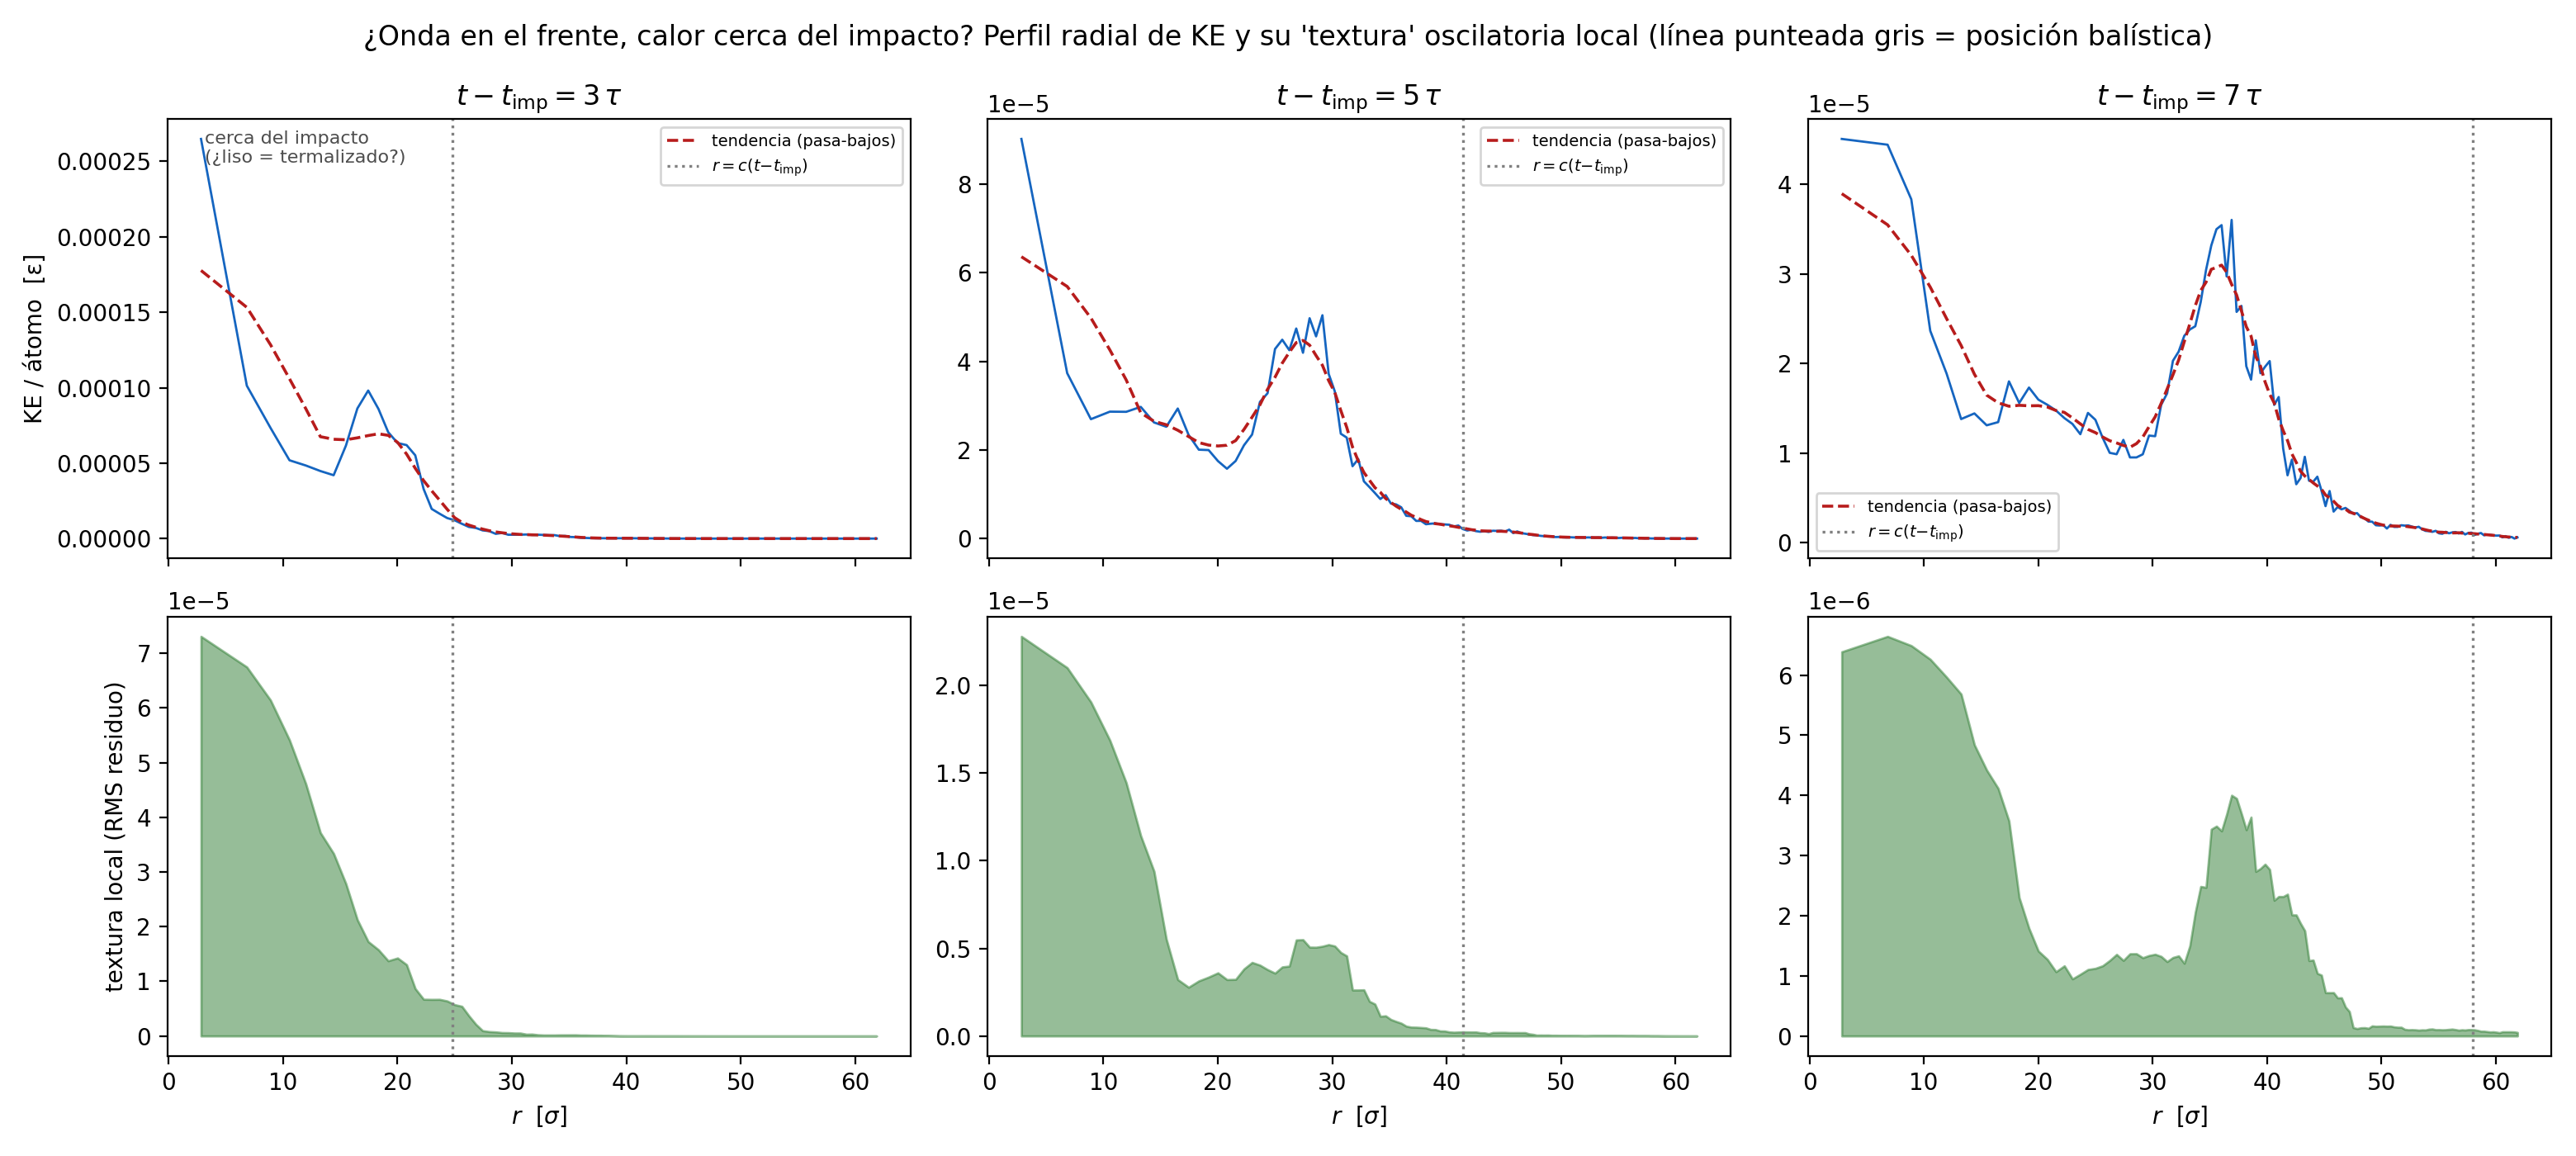
\includegraphics[width=\textwidth]{../figuras_rbef/fig_coherencia_radial.png}
\caption{Perfil radial de KE (arriba) y su ``textura'' oscilatoria local
--RMS del residuo tras restar una tendencia suavizada-- (abajo), en tres
instantes tras el impacto. La textura es alta cerca del punto de impacto
en los tres casos, con un repunte secundario justo en la posición del
frente balístico ($r=c(t-t_{\rm imp})$, línea punteada). Sobrevive el
control de sesgo por área (bins de área igual, no de ancho igual). Es la
firma de dispersión armónica (Sec.~\ref{sec:dispersion}), no de
termalización.}
\label{fig:coherencia}
\end{figure}

La red FCC no tiene relación de dispersión lineal $\omega=ck$ para todo
$k$ --solo en el límite acústico de longitud de onda larga. Los modos de
alta frecuencia viajan con menor velocidad de grupo que los modos acústicos
de baja frecuencia. Un impacto puntual excita todas las frecuencias a la
vez, superpuestas, en el punto de origen: mucha ``textura'' porque hay
muchos modos mezclados. Con el tiempo, los modos rápidos (acústicos) se
adelantan y llegan solos al frente --de ahí el repunte de textura ahí--
mientras que cerca de la fuente siguen sin separarse los modos lentos. Este
es precisamente el mecanismo que exploran las simulaciones de
\emph{wave-packet} de Schelling, Phillpot y Keblinski (2002)
\cite{Schelling2002}: generan un paquete de fonones de una rama y frecuencia
definidas en dinámica molecular y siguen su propagación balística a la
velocidad de grupo del modo, sin que la anarmonicidad (si es débil) lo
disperse --exactamente el régimen en el que probablemente estamos.

\textbf{El punto crítico:} tanto la dispersión armónica (reversible, sin
producción de entropía) como la difusión térmica real (irreversible, con
producción de entropía) pueden producir perfiles espaciales
``complicados'' que no son un simple frente nítido. \emph{Textura u
onduloso vs. liso} no distingue entre ambas. Se necesita un criterio que
sea sensible específicamente a la pérdida de coherencia de fase y
dirección, no solo a la complejidad visual del perfil.

\subsection{Un tercer régimen: sonido difuso (todavía no calor)}
\label{sec:sonido_difuso}

Hay además un régimen intermedio, bien establecido en sismología y
acústica, que conviene nombrar aparte porque el exponente $p\approx0.70$
que medimos con $r_{\rm rms}$ (Fig.~\ref{fig:frente}) también podría ser
su firma, no solo dispersión armónica pura. Cuando un pulso elástico se
dispersa \emph{muchas veces} (por fronteras de grano, defectos, o --como
aquí-- superposición de múltiples ramas y reflexiones internas), la fase
se pierde por pura complejidad de interferencia, y el campo deja de poder
describirse por su forma de onda y pasa a describirse solo por su densidad
de energía --un campo \textbf{difuso}. \textbf{Weaver (1984)}
\cite{Weaver1984} formalizó esto para placas elásticas: tras suficientes
reflexiones internas, la energía vibracional se reparte en un campo difuso
cuya evolución se describe con una ecuación de transporte radiativo
--formalmente parecida a la ecuación de calor, pero \textbf{sin que haga
falta ninguna anarmonicidad ni producción de entropía todavía}: sigue
siendo la misma energía mecánica, solo que sus muchos caminos internos ya
interfieren de forma demasiado compleja para seguirlos individualmente.
\textbf{Aki y Chouet (1975)} \cite{AkiChouet1975} identificaron el mismo
fenómeno en sismología --la ``coda'' de un terremoto, la cola larga y
decreciente de la señal sísmica después de las ondas principales, producto
de dispersión múltiple en la corteza heterogénea.

La distinción con el calor genuino de la Sec.~\ref{sec:armonico} es exacta
en el lenguaje de la Sec.~\ref{sec:segunda_ley}: un campo difuso
\emph{todavía es exergía} --sonido, no calor-- porque en principio (con
suficiente control) su energía sigue siendo recuperable como trabajo
coherente; solo parece ``aleatorio'' porque hay demasiadas trayectorias
superpuestas para seguirlas una por una, no porque la segunda ley ya haya
actuado sobre ella. El calor de Fourier, en cambio, es anergía genuina: ahí
sí la producción de entropía es irreversible. Nuestra textura alta cerca
del impacto (Fig.~\ref{fig:coherencia}) es compatible con ambas
explicaciones --dispersión armónica de modos con distinta velocidad de
grupo (Sec.~\ref{sec:dispersion}), o el comienzo de un campo difuso tipo
Weaver-- y ninguna de las dos requiere calor todavía. El criterio de la
sección siguiente distingue las tres posibilidades a la vez.

% =============================================================================
\section{El criterio correcto: isotropía de velocidades, o cuánta exergía queda}
\label{sec:criterio}
% =============================================================================

La definición operacional de ``temperatura local'' requiere \emph{equilibrio
termodinámico local}: que la distribución de velocidades en una región
pequeña sea aproximadamente isotrópica y Maxwelliana, sin una dirección
privilegiada que recuerde de dónde vino la energía. Un pulso de sonido (o
un campo difuso, Sec.~\ref{sec:sonido_difuso}, todavía) mueve los átomos
predominantemente en la dirección de propagación (para un modo
longitudinal, radialmente hacia afuera desde el impacto) --anisotropía
direccional detectable incluso si el perfil de energía ya se ve suave. Esa
anisotropía \emph{es} la exergía de la Sec.~\ref{sec:segunda_ley}: mientras
las velocidades recuerden una dirección, esa energía es en principio
extraíble como trabajo coherente (rectificable con el transductor
adecuado); una vez isotrópica, ya es anergía --calor puro, irrecuperable
más allá del límite de Carnot.

Concretamente, esto se puede medir en cada celda espacial y en cada
instante con un cociente de anisotropía,
\begin{equation}
\eta(\mathbf r,t) \equiv
\frac{\langle v_r^2\rangle - \langle v_\perp^2\rangle}
     {\langle v_r^2\rangle + \langle v_\perp^2\rangle},
\label{eq:anisotropia}
\end{equation}
con $v_r$ la componente radial (respecto al punto de impacto) y $v_\perp$
las componentes tangenciales de la velocidad de cada átomo de la celda.
$\eta\approx1$: movimiento casi puramente radial --toda la energía
cinética local es exergía, sonido en el sentido fuerte. $\eta\approx0$:
velocidades isotrópicas --el átomo ya no recuerda la dirección de la onda
que lo excitó, la energía es anergía, y ahí \emph{sí} aplica una
descripción de tipo ``calor''. Valores intermedios miden literalmente la
fracción de exergía que queda, $\mathrm{Ex}/E\sim|\eta|$: el mismo cociente
sirve para cuantificar el régimen difuso de la Sec.~\ref{sec:sonido_difuso}
(esperable $\eta$ apreciable pero menor que 1, sin necesitar $\eta=0$) y
distinguirlo tanto del sonido balístico puro ($\eta\approx1$) como del
calor genuino ($\eta\approx0$). A diferencia de la textura espacial,
$\eta$ no se confunde con dispersión armónica ni con el campo difuso: un
paquete disperso o difuso pero mecánicamente coherente sigue siendo
direccional ($\eta$ apreciable) aunque su perfil de amplitud ya no sea un
pulso nítido.

% =============================================================================
\section{Aplicación a los datos de este proyecto}
\label{sec:aplicacion}
% =============================================================================

\begin{center}
\small
\begin{tabular}{@{}p{4.4cm}p{2.9cm}p{7.3cm}@{}}
\toprule
Fuente & Resultado & Interpretación \\
\midrule
\multicolumn{3}{l}{\textit{Predicción (bibliografía, antes de mirar los datos):}} \\[2pt]
$\ell_{\rm fonón}^*$ (Kaburaki 1998, Ec.~\ref{eq:ell_kaburaki}) & $10$--$36\,\sigma$ &
  comparable a nuestra ventana limpia \\[4pt]
$\mathrm{Kn}=\ell_{\rm fonón}^*/L_{\rm limpio}$ & $\sim1$--$5$ &
  frontera balística; no debería verse calor aún \\[4pt]
\multicolumn{3}{l}{\textit{Medición (este proyecto):}} \\[2pt]
$r_{\rm frente}\propto t^p$ (umbral) & $p=1.00$--$1.06$ &
  sonido balístico, $\eta\approx1$ esperado \\[4pt]
$r_{\rm rms}\propto t^p$ (ponderado por energía) & $p\approx0.70$--$0.75$,
  estable (sin drift en 10$\tau$) & frontera de sonido difuso
  (Sec.~\ref{sec:sonido_difuso}), no necesariamente calor \\[4pt]
Textura espacial del perfil $\mathrm{KE}(r)$ & alta cerca del impacto,
  repunte en el frente & dispersión y/o campo difuso; \emph{no} evidencia
  de anergía/termalización \\[4pt]
Anisotropía de velocidad / exergía $\eta(\mathbf r,t)$ & \textbf{no medido
  todavía} & criterio correcto pendiente \\
\bottomrule
\end{tabular}
\end{center}

\textbf{Conclusión honesta:} la predicción de la bibliografía y la medición
coinciden: confirmamos con precisión sonido balístico limpio, y el número
de Knudsen calculado de forma independiente ($\mathrm{Kn}\sim1$--$5$,
Sec.~\ref{sec:kn_numerico}) explica \emph{por qué} --no es que el calor no
exista, es que nuestra ventana observable todavía no es lo bastante grande
frente al camino libre medio esperado. Lo que antes leíamos como
``ambiguo'' (textura, $p\approx0.7$) ahora tiene un lugar propio: es
probablemente el borde de la región de \textbf{sonido difuso}
(Sec.~\ref{sec:sonido_difuso}) --energía todavía mecánica y en principio
capaz de trabajo, dispersada por interferencia múltiple pero sin la
producción de entropía que exige el calor genuino. Tres regímenes, no dos:
sonido balístico ($\eta\approx1$) $\to$ sonido difuso ($\eta$ intermedio,
todavía exergía) $\to$ calor ($\eta\approx0$, anergía). Dos caminos hacia
adelante, no excluyentes:

\begin{enumerate}[leftmargin=1.4em]
\item \textbf{Medir $\eta(\mathbf r,t)$ (Sec.~\ref{sec:criterio})} sobre los
datos que ya existen (\texttt{ondas\_N79\_libre}), dentro de la ventana
limpia de $\sim7.5\tau$. Es el criterio físicamente correcto --y el único
capaz de separar sonido difuso de calor genuino-- y no requiere ninguna
simulación nueva.
\item \textbf{Extender la ventana limpia} (esponja absorbente mejor
afinada, o dominio más grande) si $\eta$ sigue apreciable en todo el rango
observable --lo que indicaría que el camino libre medio de estos fonones
excede lo que alcanzamos a ver, y que \emph{sí} hace falta más espacio/tiempo
para llegar al calor genuino, no un mejor diagnóstico.
\end{enumerate}

% =============================================================================
\begin{thebibliography}{9}

\bibitem{Kelvin1852}
W. Thomson (Lord Kelvin), \textit{On a Universal Tendency in Nature to the
Dissipation of Mechanical Energy}, Proc. R. Soc. Edinburgh \textbf{3},
139--142 (1852). Primera formulación de la segunda ley como tendencia
universal de la energía mecánica (coherente) a degradarse en calor;
el origen histórico del criterio de Gonzalo.

\bibitem{Gibbs1873}
J.W. Gibbs, \textit{A Method of Geometrical Representation of the
Thermodynamic Properties of Substances by Means of Surfaces}, Trans.
Connecticut Acad. Arts Sci. \textbf{2}, 382--404 (1873). Da forma
cuantitativa concreta a la ``energía disponible'' de Thomson (energía
libre de Gibbs).

\bibitem{Keenan1932}
J.H. Keenan, \textit{A Steam Chart for Second Law Analysis}, Mech. Eng.
\textbf{54}, 195 (1932). Introduce el término \textit{availability}
(disponibilidad) en ingeniería de turbinas de vapor.

\bibitem{Rant1956}
Z. Rant, \textit{Exergie, ein neues Wort für ``technische
Arbeitsfähigkeit''}, Forsch. Ing.-Wes. \textbf{22}, 36--37 (1956). Acuña
el término \textit{exergía}: el máximo trabajo extraíble de un sistema al
llevarlo al equilibrio con su entorno --Ec.~(\ref{eq:exergia}).

\bibitem{Weaver1984}
R.L. Weaver, \textit{Diffuse waves in finite plates}, J. Sound Vib.
\textbf{94}, 319--335 (1984). Formaliza el campo difuso (sonido disperso
por reflexión/dispersión múltiple, descrito por transporte radiativo, sin
necesitar anarmonicidad ni producción de entropía) --el régimen
intermedio de la Sec.~\ref{sec:sonido_difuso}.

\bibitem{AkiChouet1975}
K. Aki, B. Chouet, \textit{Origin of coda waves: Source, attenuation and
scattering effects}, J. Geophys. Res. \textbf{80}, 3322--3342 (1975).
Origen sismológico del concepto de campo difuso: la ``coda'' de un
terremoto, producida por dispersión múltiple en la corteza heterogénea.

\bibitem{Peierls1929}
R. Peierls, \textit{Zur kinetischen Theorie der Wärmeleitung in Kristallen},
Ann. Phys. \textbf{395}, 1055 (1929). Formulación original de la ecuación de
transporte de Boltzmann para fonones; introduce los procesos Umklapp como
mecanismo necesario para la difusión genuina de energía.

\bibitem{RLL1967}
Z. Rieder, J.L. Lebowitz, E. Lieb, \textit{Properties of a Harmonic Crystal
in a Stationary Nonequilibrium State}, J. Math. Phys. \textbf{8}, 1073
(1967). Prueba que un cristal armónico no obedece la ley de Fourier: el
flujo de calor es proporcional a $\Delta T$, no a $\Delta T/L$.

\bibitem{FPU1955}
E. Fermi, J. Pasta, S. Ulam (cálculos de M. Tsingou), \textit{Studies of
Nonlinear Problems I}, Los Alamos report LA-1940 (1955); publicado en
\textit{Collected Papers of Enrico Fermi} (Univ. of Chicago Press, 1965).
El experimento numérico fundacional que mostró que la anarmonicidad débil
no basta para termalizar en tiempos razonables (recurrencia casi completa
tras 157 períodos).

\bibitem{LLP2003}
S. Lepri, R. Livi, A. Politi, \textit{Thermal conduction in classical
low-dimensional lattices}, Phys. Rep. \textbf{377}, 1--80 (2003). Revisión
extensa de cuándo se recupera la ley de Fourier y cuándo el transporte de
calor sigue siendo anómalo (conductividad divergente) incluso con
anarmonicidad presente.

\bibitem{Schelling2002}
P.K. Schelling, S.R. Phillpot, P. Keblinski, \textit{Phonon wave-packet
dynamics at semiconductor interfaces by molecular-dynamics simulation},
Appl. Phys. Lett. \textbf{80}, 2484 (2002). Método de dinámica molecular
directamente análogo al usado aquí: sigue un paquete de fonones localizado
y su transporte balístico/dispersivo.

\bibitem{Cahill2003}
D.G. Cahill, W.K. Ford, K.E. Goodson, G.D. Mahan, A. Majumdar, H.J. Maris,
R. Merlin, S.R. Phillpot, \textit{Nanoscale thermal transport}, J. Appl.
Phys. \textbf{93}, 793--818 (2003). Revisión del número de Knudsen y el
cruce balístico-difusivo en sistemas nanométricos, con ejemplos
experimentales (grafeno suspendido, entre otros).

\bibitem{Kaburaki1998}
H. Kaburaki, J. Li, S. Yip, \textit{Thermal Conductivity of Solid Argon by
Classical Molecular Dynamics}, MRS Online Proc. Lib. \textbf{538}, 503--508
(1998). Camino libre medio de fonones acústicos en argón sólido
Lennard-Jones vía Green-Kubo ($\approx12.2$~nm a 10~K, $\approx3.4$~nm a
40~K) --el mismo potencial y los mismos parámetros de argón que este
proyecto; da el número de Knudsen concreto de la Sec.~\ref{sec:kn_numerico}.

\bibitem{Hunter1957}
S.C. Hunter, \textit{Energy absorbed by elastic waves during impact}, J.
Mech. Phys. Solids \textbf{5}, 162--171 (1957). Calcula, en el límite
puramente elástico/ondulatorio (sin ningún componente difusivo), la energía
radiada como ondas elásticas en el impacto de una esfera sobre un
semi-espacio; predice que esa fracción es pequeña cuando $v_{\rm imp} \ll
c_{\rm sonido}$ --consistente con nuestro $\alpha_{\rm surf}$ relativamente
chico frente a los otros canales.

\bibitem{AshcroftMermin}
N.W. Ashcroft, N.D. Mermin, \textit{Solid State Physics} (Saunders College,
1976). Tratamiento estándar de posgrado de fonones, dispersión, y
conductividad térmica (ya citado en \texttt{equiparticion\_y\_virial.tex}).

\end{thebibliography}

\end{document}
